\documentclass[12pt]{article}
\usepackage[utf8]{inputenc}
\usepackage{graphicx}
\usepackage[brazil]{babel}
\usepackage{amsmath, amssymb}
\usepackage{geometry}
\geometry{a4paper, margin=2.5cm}
\title{BCC325 – Prova 1 \\ Inteligência Artificial}
\author{Universidade Federal de Ouro Preto}
\date{}

\begin{document}

\maketitle

\vspace{0.5cm}

\textbf{Instruções:} Responda às questões a seguir com clareza e objetividade. Justifique todas as suas respostas sempre que possível. 

\begin{enumerate}

\item (1,0 pt) No contexto de busca em espaços de estados, explique:
\begin{enumerate}
    \item O que caracteriza um problema de busca.
    \item Quais são os componentes fundamentais de um problema de busca.
\end{enumerate}

\item (1,0 pt) Relacione espaços de estados e grafos. Em seguida, descreva os elementos de um problema de busca quando representado como grafo.

\item (1,5 pt) Apresente o algoritmo genérico de busca e explique como ele pode ser adaptado para busca em profundidade e busca em largura. Mostre as diferenças principais entre essas duas estratégias quanto a:
\begin{itemize}
    \item estrutura de dados usada;
    \item tipo de solução encontrada;
    \item complexidade de tempo e espaço.
\end{itemize}


\item (2,0 pt) Apresente, passo a passo, a execução da sua implementação do algoritmo de busca em largura em uma matriz 4×4 com início em $(0,0)$ e objetivo em $(3,3)$. Represente a fronteira a cada iteração. Considere apenas células livres (0) e bloqueios (1). Você pode criar o exemplo.

\item (1,5 pt) Resolva as questões a seguir nos labitintos abaixo:

Sabendo que o agente deve se mover na ordem para cima, baixo, esquerda ou direita:

\begin{enumerate}
    \item Numere os nós expandidos por uma busca em profundidade. Ordem das ações: cima, esquerda, direita, baixo. Assuma poda de ciclos.
    \item Numere os nós expandidos por uma busca de menor custo primeiro, assumindo custo unitário.
    %\item Numere os nós expandidos por uma busca gulosa utilizando distância de Manhattan até o objetivo como heurística.
    %\item Numere os nós expandidos pelo algoritmo A* usando custo e heurística de Manhattan.
\end{enumerate}

\begin{figure}[h]
\centering
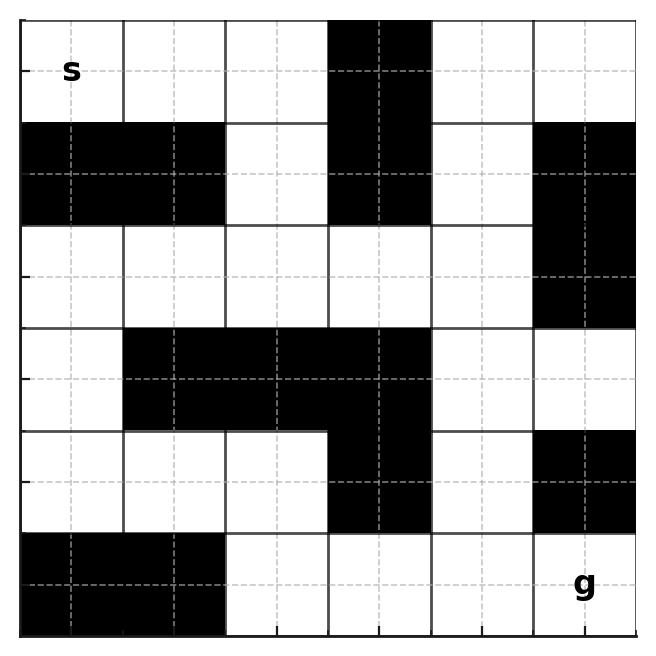
\includegraphics[width=0.6\textwidth]{labirinto_exemplo_bw.png}
\caption{Labirinto para a busca em Profundidade}
\end{figure}

\begin{figure}[h]
\centering
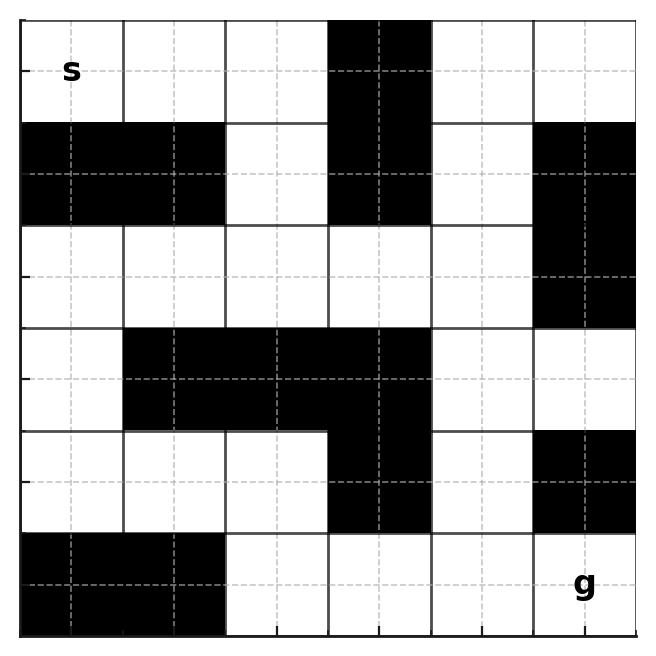
\includegraphics[width=0.6\textwidth]{labirinto_exemplo_bw.png}
\caption{Labirinto para a busca em Largura}
\end{figure}

\end{enumerate}

\end{document}
